%------------------------------------------------------------------------------
% Template file for the submission of papers to IUCr journals in LaTeX2e
% using the iucr document class
% Copyright 1999-2009 International Union of Crystallography
% Version 1.4 (11 May 2009)
%------------------------------------------------------------------------------

\documentclass[final]{iucr}              % DO NOT DELETE THIS LINE

     %-------------------------------------------------------------------------
     % Information about the type of paper
     %-------------------------------------------------------------------------
     \paperprodcode{a000000}      % Replace with production code if known
     \paperref{xx9999}            % Replace xx9999 with reference code if known
     \papertype{FA}               % Indicate type of article
                                  %   FA - research papers (full article)
                                  %   SC - short communications
                                  %   LA - lead article
                                  %   FE - feature articles
                                  %   ST - structural communications
                                  %   XC - crystallization communications


     \paperlang{english}          % Can be english, french, german or russian
     %-------------------------------------------------------------------------
     % Information about journal to which submitted
     %-------------------------------------------------------------------------
     \journalcode{J}              % Indicate the journal to which submitted
                                  %   A - Acta Crystallographica Section A
                                  %   B - Acta Crystallographica Section B
                                  %   C - Acta Crystallographica Section C
                                  %   D - Acta Crystallographica Section D
                                  %   E - Acta Crystallographica Section E
                                  %   F - Acta Crystallographica Section F
                                  %   J - Journal of Applied Crystallography
                                  %   S - Journal of Synchrotron Radiation
          %--------------------------------------------------------------------
          % The following entries will be changed as required by editorial staff
          %--------------------------------------------------------------------
     \journalyr{2010}
     \journaliss{1}
     \journalvol{65}
     \journalfirstpage{000}
     \journallastpage{000}
     \journalreceived{0 XXXXXXX 0000}
     \journalaccepted{0 XXXXXXX 0000}
     \journalonline{0 XXXXXXX 0000}
  
  
\newif\ifdograph
\dographtrue % DO keep the graphs.
%\dographfalse % DONT put graphs - makes things faster

\usepackage{ifpdf}

\usepackage{graphicx}
\DeclareGraphicsExtensions{.eps,.ps,.bmp,.tif,.tiff,.tga}  
\graphicspath{{eps/}}

\usepackage{gensymb} %General symbols
\usepackage[version=3]{mhchem} %For chemical formulae
\usepackage{subfigure} 
 

%quick angstrom define
\newcommand{\ang}{$\mathrm{\AA} $}
%\newcommand{\th}[0]{\superscript{th}}

\begin{document}                  % DO NOT DELETE THIS LINE

 %-------------------------------------------------------------------------
 % The introductory (header) part of the paper
 %-------------------------------------------------------------------------

\title{CrystalPlan: an Experiment Planning Tool for Crystallography}

\shorttitle{CrystalPlan: an Experiment Planning Tool}

 % Authors' names and addresses. Use \cauthor for the main (contact) author.
 % Use \author for all other authors. Use \aff for authors' affiliations.
 % Use lower-case letters in square brackets to link authors to their
 % affiliations; if there is only one affiliation address, remove the [a].

\cauthor[]{Janik}{Zikovsky}{zikovskyjl@ornl.gov}{address if different from
\aff}
\author[]{Peter}{Peterson}
\author[]{Xiaoping}{Wang}
\author[]{Matthew}{Frost}
\author[]{Christina}{Hoffmann}

\aff[]{Spallation Neutron Source, Oak Ridge National Laboratory, P.O. Box 2008
MS-6477, Oak Ridge, TN 37831-6477
\country{USA}}

 % Use \shortauthor to indicate an abbreviated author list for use in
 % running heads (you will need to uncomment it).

\shortauthor{Zikovsky et al.}




\maketitle                        % DO NOT DELETE THIS LINE 

\begin{synopsis}
Describes CrystalPlan, a software program for the automatic creation of 
crystallography experiment plans for time-of-flight diffractometers.
\end{synopsis}

\begin{abstract}
Beam time at large user program based x-ray and neutron scattering facilities is
in high demand and always at a premium. CrystalPlan, a highly efficient
experiment planning software has been developed to maximize the use of available
beamtime per sample per experiment. 
This program can calculate and optimize the data coverage of a crystal in
reciprocal space in a single-crystal diffraction time-of-flight experiment.
CrystalPlan can help a user build an experiment plan that will acquire the most
unique data possible, with sufficient coverage but limited redundancy, therefore
increasing scientific productivity. 
A user friendly GUI (Graphical User Interface) including a 3D viewer, an
automated coverage optimizer, and an option to reorient the crystal for the measurement 
of selected $hkl$s on specific detector positions 
are among its useful features. 
A sample use case of the program with the TOPAZ beamline at SNS will be
presented. 
\end{abstract}



%-------------------------------------------------------------------------
%-------------------------------------------------------------------------
%-------------------------------------------------------------------------
\section{Introduction}

The TOPAZ beamline at the Spallation Neutron Source (SNS) at Oak Ridge National
Laboratory (ORNL), currently finishing commissioning, is a neutron
time-of-flight Laue diffractometer with high wavelength (time) resolution. It
is designed to acquire single-crystal diffraction data of small-to-moderate sized unit cells with  high
throughput. The final design calls for an array of 48 detectors covering
approximately half of $4\pi$ steradians. However as of this writing, only 14 of
the 48 detectors are installed, giving only a sixth of $4\pi$ steradian
coverage. To have sufficient data for a reliable structure solution and  
refinement, an experimenter will typically want to measure $ > 85\%$ of the
unique reflections within a certain range of d-spacings. However, TOPAZ's wide 
wavelength band combined with its complex geometry makes it difficult to come up
with  an effective set of sample orientations that will cover all the required
reflections without unnecessary redundancy. 


Existing diffraction experiment planning software programs (for example,
CrysAlis Pro from Oxford Diffraction; COSMO from Bruker AXS) were designed for
X-ray experiments where the crystal is rotated stepwise through the Bragg
diffraction condition using a single incident wavelength, 
resulting in a large number of sample orientations.
These programs are not suitable for TOPAZ, since as a time-of-flight instrument
(time-resolved Laue), it is collecting data from a wide
bandwidth of incident neutrons, thus contracting the Ewald sphere through the
reflection condition while keeping the crystal stationary, as described in
\cite{Schultz94,Wilson00}.
 Additionally, this means that relatively few sample
orientations are needed to complete a measurement: whereas an X-ray measurement might have
hundreds or thousands of individual frames, a TOPAZ run may have as few as 10
to cover the same volume of reciprocal space.


The goal of CrystalPlan was to make an easy-to-use software tool to aid users in
planning their experiments. By quickly making an experimental plan that will be
tailored to the needs of the scientist (enough reflections measured for a structure
analysis), but without spending time collecting redundant data, CrystalPlan will
greatly increase the scientific productivity and throughput of TOPAZ and other
similar beamlines. Users will be able to measure samples highly efficiently,
allowing them to explore parameters such as temperature and pressure more fully.
 
%---------------------------------------------------------------------------------------
%---------------------------------------------------------------------------------------
%---------------------------------------------------------------------------------------
\section{Architecture}

CrystalPlan is designed with these capabilities:

\begin{itemize}
  \item Load a geometry file for a specific instrument (using a generic,
  flexible file format).
  \item Calculate the orientation of a crystal at different goniometer settings.
  \item Calculate the coverage of these orientations in reciprocal space,
  in volume and for single reflections.
  \item Take into account crystal Bravais lattice symmetries and the higher
  redundancy of higher space groups.
  \item Optimize the experiment plan automatically.
  \item Compare predicted and actual measurement of reflections.
\end{itemize}

\subsection{Instrument Configuration}

CrystalPlan currently supports area detectors with flat faces and arbitrary
rectangular dimensions; this reflects the detector types in use at SNS (Anger
cameras and 8-pack $^3$He tube detectors), but the software could easily be
extended for more complicated detector shapes as needed. The detector configuration is loaded from
a text file containing the location, size, orientation and number of pixels of
each detector. Other settings to be adjusted for an instrument include the
detectable range of neutron/x-ray wavelength.


\subsection{Sample Orientation}

CrystalPlan can accomodate a variety of sample
orientation goniometers. A base Goniometer class (in the object-oriented
programming sense) is subclassed for specific types of goniometers, allowing a
unified interface. This base class acts as a \emph{universal goniometer},
which uses the conventional Eulerian goniometer angles of
$\phi$, $\chi$, $\omega$ as defined in \cite{busing67}.
Each class inheriting from the base Goniometer can convert
the desired $\phi$, $\chi$, $\omega$ angles to the internal motor positions it requires. 
The class hierarchy allows for goniometer limitations: for example, TOPAZ is
currently equipped with a goniometer where $\chi$ is fixed at 45 degrees
(at $\omega$ to the incident beam). CrystalPlan handles this by limiting the
sample orientation angles accessible to the user to $\phi$ and $\omega$.
    
The sample unit cell and orientation is typically determined by the data
collection/reduction software. In our case, from an initial data set, the data
analysis program ISAW (Integrated Scattering Analysis
Workbench \cite{Mikkelson05}) provides us with the unit cell of the sample (via
the B matrix) and the sample mounting orientation (U matrix).
The combined UB matrix is then saved to a
text file along with the lattice parameters. 
CrystalPlan can load this UB matrix file and uses it for reciprocal coverage
calculations and optimization.
    
  
\subsection{Reciprocal Space Representation}

The reciprocal space to be measured is divided into a cubic 3D matrix 
of {\bf Q}-space (with {\bf Q} defined as $\frac{2\pi}{d}$). 
The user specifies the minimum d-spacing ($d_{min}$, in \ang) 
that he or she is interested in, defining the limit
$Q_{max} = \frac{2\pi}{d_{min}}$ of the modeled volume. There is no lower limit
on {\bf Q}.

The resolution of the 3D matrix is also specified
(in \ang$^{-1}$), which determines the number of points (voxels or volumetric pixels) to be modeled. Available machine memory
limits the resolution that can be achieved in practice.

Each point of the reciprocal space 3D matrix holds an integer representing the 
number of times that voxel of {\bf Q}-space has
been measured -- this is the total coverage matrix. To speed up the
calculation of the total, a coverage matrix for each sample orientation is 
calculated and saved in memory and the total coverage
matrix can be computed by simply adding multiple 3D matrices corresponding to each sample orientation. 
 
\subsection{Calculating Coverage of One Sample Orientation}

For each sample orientation, a rotation matrix combining the sample's mounting
orientation (the U matrix loaded from ISAW) and the goniometer rotation matrices
($\Phi$, $\chi$, $\Omega$) is computed. The coverage in reciprocal space is
computed in this way: for each pixel in the face of a detector, the direction of
the scattered beam is known. Then, two incident beam vectors are considered,
corresponding to the $\lambda_{min}$ and $\lambda_{max}$ wavelength limits
of the detectors and/or source. The scattered beam direction and the two possible incident beam vectors
are used to find two $\overrightarrow q$ vectors; these point in the
same direction. At the high wavelength limit we find $\overrightarrow q_{min}$,
and the low wavelength limit corresponds to $\overrightarrow
q_{max}$. Since the instrument has a wavelength bandwidth, we fill in the 3D {\bf Q}-space
matrix by filling all points from $\overrightarrow q_{min}$ to the 
$\overrightarrow q_{max}$, for all pixels in the face of the detector.
A typical wavelength band for TOPAZ is from 0.5 to 3.6 \ang.
This readily defines a volume of coverage, as shown schematically in
two dimensions in Figure \ref{fig:ewald_fig}.


To reduce memory usage yet allow for quickly trying different detector
configurations, the 3D matrix of each sample orientation is saved as a 32- or
64-bit integer, with each bit representing a particular detector. A simple
binary mask can then be applied to quickly compute the coverage if some
detectors are disabled, for example.          




\subsection{Crystal Parameters and Single Reflection Coverage}

Crystal lattice parameters (lengths $a$, $b$, $c$ and angles $\alpha$, $\beta$,
$\gamma$) are typed in or loaded from the ISAW UB matrix file. CrystalPlan then
generates a list of $hkl$ reflections with d-spacings larger than the $d_{min}$
specified. For each sample orientation being simulated and for each reflection, a function calculates at
what wavelength $\lambda$ and in which direction it scatters. If $\lambda$ 
is within range of the limits of the instrument, the beam direction is projected
onto each detector face to determine where, on each detector surface, it will be
measured. 
 
Each $hkl$ reflection is a separate object that holds all predicted
recordings, including which detector measured it, at what (x,y) position on the
detector face, at what wavelength, and for which sample orientation. These data
are used to graphically display coverage and calculate statistics such as
redundancy. 



\subsection{Crystal Symmetry}
\label{sec:symm}
The crystal's point group symmetry can
be entered along with its lattice parameters.
This information is then used to
calculate the increased measurement redundancy for higher symmetries
\cite{giacovazzo92}. 
A list of $n$ $3\times3$ multiplication matrices is generated based on the point group; 
all $hkl$ vectors are multiplied by
these matrices to find the $n$ equivalent $hkl$ reflections; for example, for
orthorhombic (mmm) symmetry, $n=8$; therefore 8 multiplication matrices are
generated that multiply $hkl$ to give $\pm h$, $\pm k$, $\pm l$.              

Each reflection is tracked separately, but a primary
$hkl$ is identified that points to a list of equivalent $hkl$'s when the
crystal symmetry is known.
The interactive GUI displays either all $hkl$, ignoring crystal symmetry; or
combines them to display only the primary $hkl$'s, and calculates the
redundancy by summing all measurements on all equivalent $hkl$'s.

In volume coverage mode, a 4D array is generated where the first 3 dimensions
correspond to {\bf Q}-space, and the $4^{th}$ dimension is a list of $n$
entries. Each entry in the $4^{th}$ dimension points to a voxel that is an
equivalent due to crystal symmetry. This allows CrystalPlan to quickly compute a volume coverage
map that takes into account crystal symmetry and the resulting redundancy: at
each voxel, all $n$ equivalent voxels are checked to see if any of them were
measured.



\subsection{Automatic Coverage Optimizer}

CrystalPlan allows the user to manually enter lists of sample orientations to
simulate and graphically display the coverage in reciprocal space;
however, finding an optimal plan by trial and error is in general 
time consuming and only feasible for an experienced crytallographer.
To make the process more efficient, CrystalPlan includes an Automatic
Coverage Optimizer, which takes as its inputs the desired number of sample
orientations and uses a genetic algorithm to find a solution that satisfies a
user-specified coverage criterion (for example, the user may ask for $85\%$ of 
Bragg reflections to be measured, or for $90\%$ of {\bf Q}-volume). 

Genetic algorithms have been covered in the literature before, see e.g.
\cite{Goldberg89}. In this application, the genes
consist of goniometer angles. For instance, if a goniometer has freedom in 3 angles and the user
requests 10 different sample orientations, then each individual has 30 genes.
The initial population is created randomly and is made to evolve using mutations
and crossover. Individuals whose goniometer angles turn out to be impossible to
reach or beyond set limits are eliminated. For each individual set of sample
orientations, the coverage statistics are computed (taking crystal symmetry into
account if desired), and this is used as the fitness of the given individual in
the normal genetic algorithm process. The best individuals are saved after each
cycle. The simulation has succeeded once the desired value is reached or
exceeded or the maximum number of cycles was calculated.    

The Automatic Coverage Optimizer can find an acceptable solution (if any is
possible) in times ranging from a few seconds to several minutes, depending on
the difficulty of the problem and the computing hardware. Given that at a
neutron facility, a measurement of a single orientation may take a few
hours, this feature can result in significant beam-time savings.           




%---------------------------------------------------------------------------------------
%---------------------------------------------------------------------------------------
%---------------------------------------------------------------------------------------
\section{Implementation}




\subsection{Language and Libraries}

The program was designed to be cross-platform, and to run equally well on Linux,
Mac OS and Windows, although Linux is our primary target operating system. Another
design goal was to use open-source software and toolkits as much as possible. 

To this end, CrystalPlan was written in Python \cite{python}, a powerful, open,
cross-platform scripting language. Python was chosen for its ease of cross-platform deployment, and for
its attractive language features. The numpy and scipy libraries (two
open-source, commonly installed Python libraries) were used for many of the
calculations \cite{numpy,scipy}. The most time-critical calculations
were also written with inline C code, which increases the computation speed by
up to $400\times$ as compared with the pure Python version (which can still be
used, in case of incompatibilities).

\subsection{Code Layout}

The calculation code of CrystalPlan is placed in a model layer and kept
completely separate from eventual GUI elements, using a Model/View-Controller
architecture \cite{Gamma95}. This makes it possible to run calculations using
Python scripts, if desired. Unit tests for each part of the calculations are used to ensure
consistent results on different platforms and  systems.     
  

\subsection{Graphical User Interface}

\subsubsection{Design.}

An attractive and easy-to-use GUI was considered an important part of
CrystalPlan, since the program is meant to be used interactively as a guide to
the experimenter whether new or experienced. This requires intuitive GUI
interfaces and workflows.
The user interface was written using wxPython
\cite{wxPython}, a mature cross-platform GUI toolkit, as well as the Enthought
Traits GUI. Some of the 2D plots use matplotlib \cite{matplotlib},  and the 3D
visualization elements use the Mayavi2 toolkit for Python \cite{mayavi}, itself
based on VTK \cite{VTK}. All of these libraries are  open-source.

\subsubsection{Main Program Workflow.}
A screenshot of the main window GUI is shown in Figure \ref{fig:screenshots}.
The main window consists of a series of tabs, with workflow proceeding
intuitively from left to right:

\begin{itemize}
  	\item {\bf Q}-Space tab: define the volume of interest (minimum d-spacing)
  	and resolution of reciprocal space. 
 	\item Detectors tab: load instrument detector geometry
files, and enable or disable individual detectors. 
	\item Goniometer tab: to choose the
goniometer and degrees of orientation freedom of the sample.
  	\item Sample tab: enter or load the crystal's lattice parameters and UB
  matrix.
  	\item Try an Orientation tab: interactively rotate a sample and observe the
  changes in coverage in real-time.
  	\item Add Orientations tab: type in a list of sample orientation angles to
  add to the experiment plan.
 
  	\item Experiment Plan tab: a list of the previously calculated sample
orientations. Here you can manage the orientations you will use in the experiment: add,
delete, or temporarily disable them to see the effect on coverage. Once
complete, the plan can be sent to the SNS/TOPAZ data acquisition computers in
order to begin a run \cite{SNSDAS}.
    
\end{itemize} 



\subsubsection{Reciprocal Space Coverage Visualization.}
Figure \ref{fig:volume_view}a) shows a screenshot of the reciprocal space
coverage 3D interface. The 3D view can represent {\bf Q}-space in two ways: volume coverage, or single-reflection
coverage. The view shown can be rotated, translated or zoomed using the mouse or
keyboard.

The volume coverage shows a solid isosurface representing the volume measured at
least once. Redundant regions can also be shown using semi-transparent
isosurfaces; or the coverage can be inverted, showing non-measured volumes only;
or slices between user-selectable $q_{min}$ and $q_{max}$.        

The reflections view (Figure \ref{fig:refl_view}a) displays each $hkl$ as a
small sphere; the color of which indicates the number of times the $hkl$ is
predicted to be measured in the current experiment plan.        

Both views can take into account crystal symmetry in their display using the
techniques described previously in Section \ref{sec:symm}.
The volume coverage (Figures \ref{fig:volume_view}b) fills in the sphere of
coverage; 
whereas the single reflection view (Figure \ref{fig:refl_view}b) leaves only
the primary reflections (one eight of the total, in this example).
 
Finally, both views display coverage statistics in the lower right
corner, showing the percentage of volume (or of the number of reflections) measured,
as well as the proportion of redundancy (voxels or reflections measured 2 or more
times). 

\subsubsection{Single Reflection View.}
Figure \ref{fig:single_reflection} shows a screenshot of the GUI allowing one to
observe in detail the predicted measurements of a particular reflection, by clicking
in the 3D view or by typing in the $hkl$ values. The position on the detector
and wavelength of measurement are displayed. An additional window (not shown) allows the user to place the reflection on a particular
position on a detector by automatically finding the necessary sample orientation
angles. This is used, for example, to center important reflections or diffraction
directions in the most sensitive part of a detector.


%---------------------------------------------------------------------------------------
%---------------------------------------------------------------------------------------
%---------------------------------------------------------------------------------------

\section{Sample Use Case}

As part of the TOPAZ beamline commissioning process, a natrolite
(\ce{Na2Al2Si3O10} $\cdot$ \ce{2H2O}) single crystal was measured on a fixed
$45\degree\ \chi$ goniometer at room temperature and ambient atmosphere, with a
wavelength range from $\sim0.5$ \ang\ to $3.5$ \ang.
An initial short event file (each neutron detection event is saved with its
time-of-flight and position) was processed using ISAW to determine the UB
matrix and cell parameters of the crystal.

The resulting UB matrix was loaded into CrystalPlan, where the Automatic
Coverage Optimizer was used to generate an experiment plan with 8 sample
orientations (Figure \ref{fig:natrolite_gui}a) that covered 97\% of the reflections,
taking into account the crystal Laue symmetry (orthorhombic or mmm) (Figure
\ref{fig:natrolite_gui}b). The eight orientations were run
unattended overnight.

Reflections were integrated using ISAW, and the resulting file was
loaded into CrystalPlan for comparison. The predicted and actual measurement
positions on each detector face were compared for the 554 integrated reflections
found. Good agreement was found; the root-mean-square difference between the
predicted and actual measurement wavelength was only 0.016 \ang. The offsets in the reflection
position were plotted, which helped show that the main contributor to this error
was a slight misalignment of the goniometer.

%NOTE: Check on this misalignment of goniometer business - is that really the
% cause?

CrystalPlan was also successfully used in a similar way during experiments run
on the TOPAZ instrument by Yuri Janssen from State University of New York, Stony
Brook, and Henrik Clausen from University of Aarhus, Denmark. 

%---------------------------------------------------------------------------------------
%---------------------------------------------------------------------------------------
%---------------------------------------------------------------------------------------

\section{Conclusions and Future Development}

We have described CrystalPlan, a software program designed to quickly produce
efficient experiment plans for wide bandwidth time-of-flight Laue
diffractometers. This program will help increase scientific productivity at SNS
beamlines such as TOPAZ. With some relatively minor modifications, the program
could also be adapted for use at reactor sources. Monochromatic diffractometers
could be handled by adding support sweeps consisting of many motor positions;
Laue diffractometers on a constant intensity beam would requiring
detecting and removing reflections with chromatic overlap.

One planned future development for CrystalPlan include extending the software
to help predict coverage in inelastic neutron scattering experiments. Another
desired feature is the introduction of feedback loops to help determine the
right time to end data acquisition at a particular sample orientation.
CrystalPlan would interface with data analysis software such as ISAW and use
recently developed capabilities for real-time data analysis to monitor
the  signal to noise ratio on particular reflections. When the signal intensity
becomes sufficient, the sample will automatically be moved to the next sample
orientation, further adjusting data acquisition time for each specific sample.
Combined with advanced sample changers coming on-line at TOPAZ, this will allow
for extremely efficient, unattended and automated data acquisition.





















     % Appendices appear after the main body of the text. They are prefixed by
     % a single \appendix declaration, and are then structured just like the
     % body text.

%\appendix
%\section{Appendix title}

%Text text text text text text text text text text text text text text
%text text text text text text text.

     %-------------------------------------------------------------------------
     % The back matter of the paper - acknowledgements and references
     %-------------------------------------------------------------------------

     % Acknowledgements come after the appendices

\ack{Acknowledgements}

This research is supported by UT Battelle, LLC under Contract No.
DE-AC05-00OR22725 for the U.S. Department of Energy, Office of Science.



     % References are at the end of the document, between \begin{references}
     % and \end{references} tags. Each reference is in a \reference entry.
\bibliographystyle{iucr}     
\bibliography{crystalplan}   

%\begin{references}
%\reference{Author, A. \& Author, B. (1984). \emph{Journal} \textbf{Vol}, 
%first page--last page.}
%\end{references}

 %-------------------------------------------------------------------------
 % TABLES AND FIGURES SHOULD BE INSERTED AFTER THE MAIN BODY OF THE TEXT
 %-------------------------------------------------------------------------

 % Simple tables should use the tabular environment according to this
 % model



 % Postscript figures can be included with multiple figure blocks

\begin{figure}
\caption{2D Ewald construction showing reciprocal-space detector coverage
for a wide-bandwidth Laue diffractometer. The smaller blue circle represents the
$1/\lambda_{max}$ limit of measurement, with the larger green circle
representing $1/\lambda_{min}$. The origin of reciprocal space (000) is common to both
spheres, but the ``virtual" sample position in the construction (S1 or S2)
depends on $\lambda$. The angular coverage of the detector is represented by the dashed
wedge, and projects an arc onto each sphere of radius $1/\lambda$. The
red wedge between the two $\lambda$ is built by drawing straight lines between
the $q_{min}$ and $q_{max}$ limits for each pixel on the detector face, giving the
volume in reciprocal space that is measured at a single sample oriention. }

\ifdograph
  \includegraphics[width=3.5in]{ewald_fig.ps}
\fi
     
\label{fig:ewald_fig} 
\end{figure} 
 
  
\begin{figure}
\caption{Screenshot of the main GUI window. Six more interface windows (not
shown) are presented to the user when he or she clicks on the tabs at the
top of the main window.}
\ifdograph
  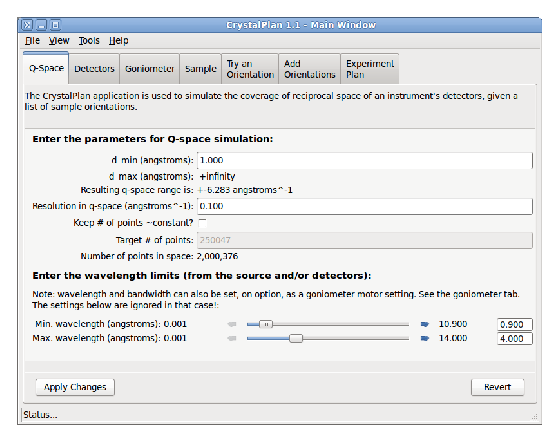
\includegraphics{main_gui}
\fi
\label{fig:screenshots}
\end{figure}
 



\begin{figure}
\caption{Sample screenshot showing the 3D view of the predicted coverage of
reciprocal space volume for 3 sample orientations and 14 detectors on TOPAZ,
from 0.9 \ang\ to 4.0\ang: a) without crystal symmetry, 17\% coverage; b) with crystal symmetry (mmm 8-fold
symmetry), coverage increases to 65\%. The area plot at the bottom shows the
measured percentage of reciprocal volume as a function of $q$; the
color indicates the redundancy (cyan: 1, green: 2, yellow: 3, orange: 4). }
\ifdograph
  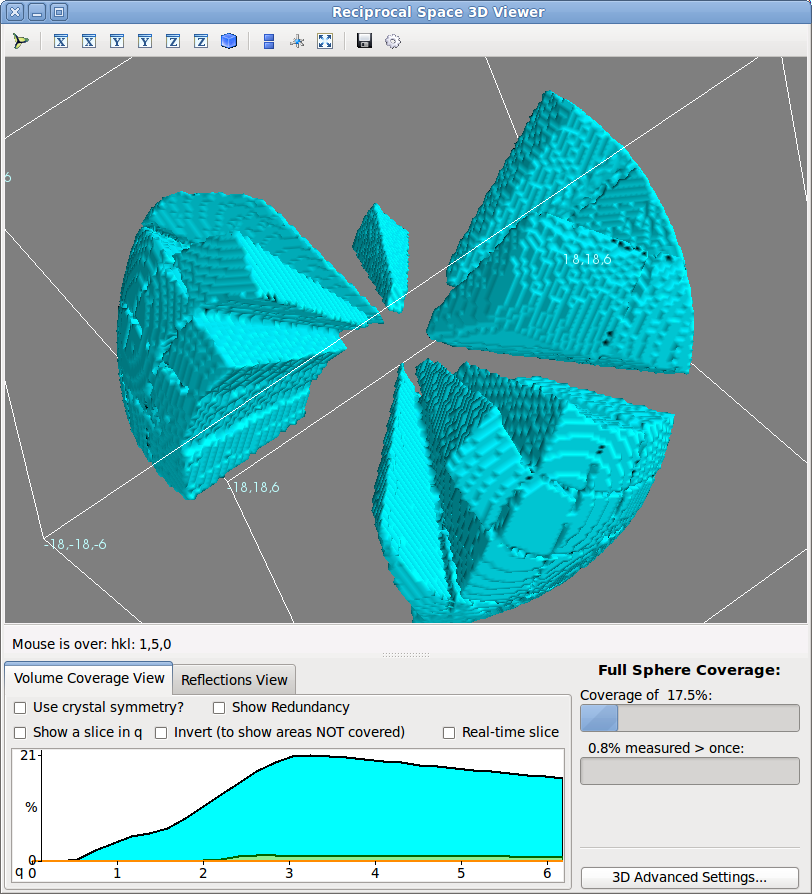
\includegraphics{volume_nosym} 
\fi
a)
\ifdograph
  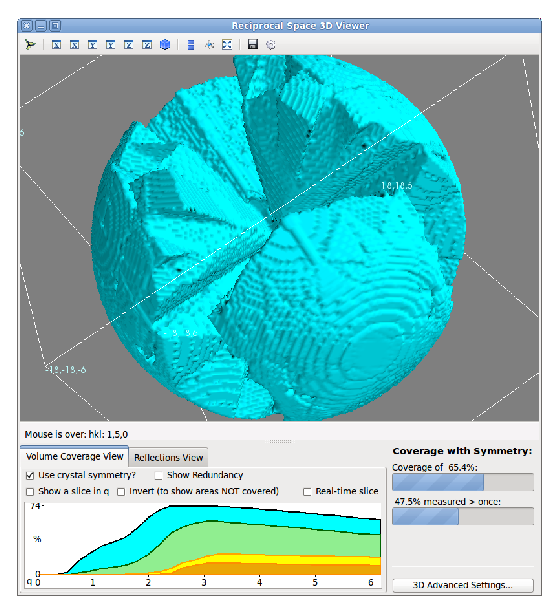
\includegraphics{volume_sym}
\fi
b)
\label{fig:volume_view} 
\end{figure}


\begin{figure}
\caption{Sample screenshot showing the 3D view of single-crystal reflection
measurements. Each sphere represents an $hkl$ reflection, color-coded to indicate the
number of measurements (dark blue: 0, cyan: 1, green: 2, yellow: 3, red: 4 or
more). a) without crystal symmetry, 2375 of 9481 reflections are measured, or
25\%. b) with crystal symmetry, 1276 of 1427 primary reflections are measured, or
89\%, and redundancy is also increased. }
\ifdograph
  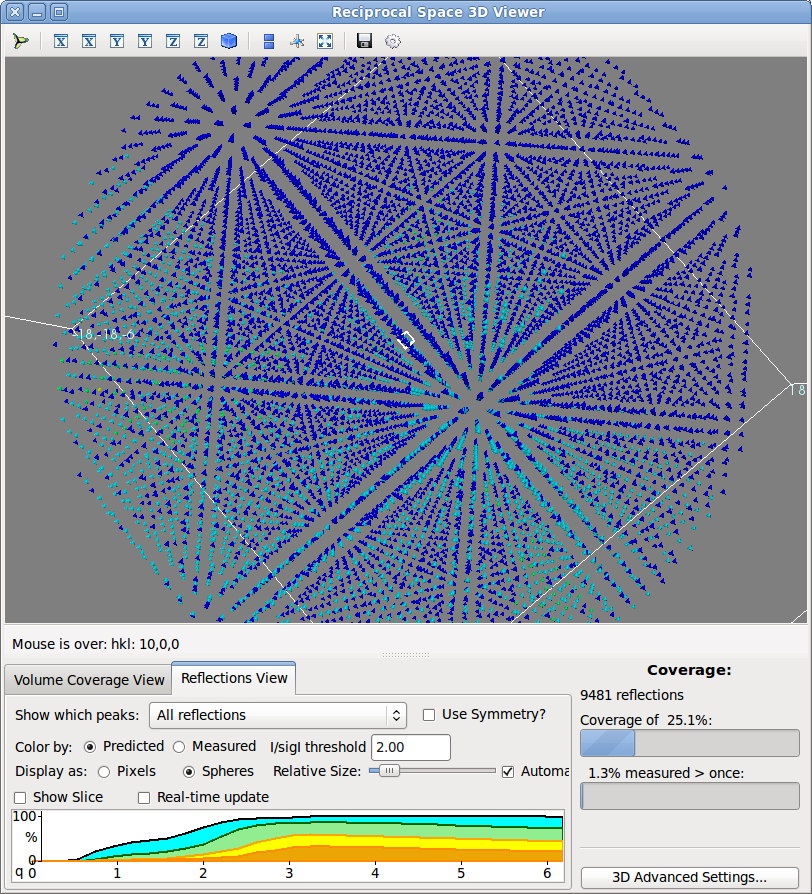
\includegraphics{refl_nosym} 
\fi
a)
\ifdograph
  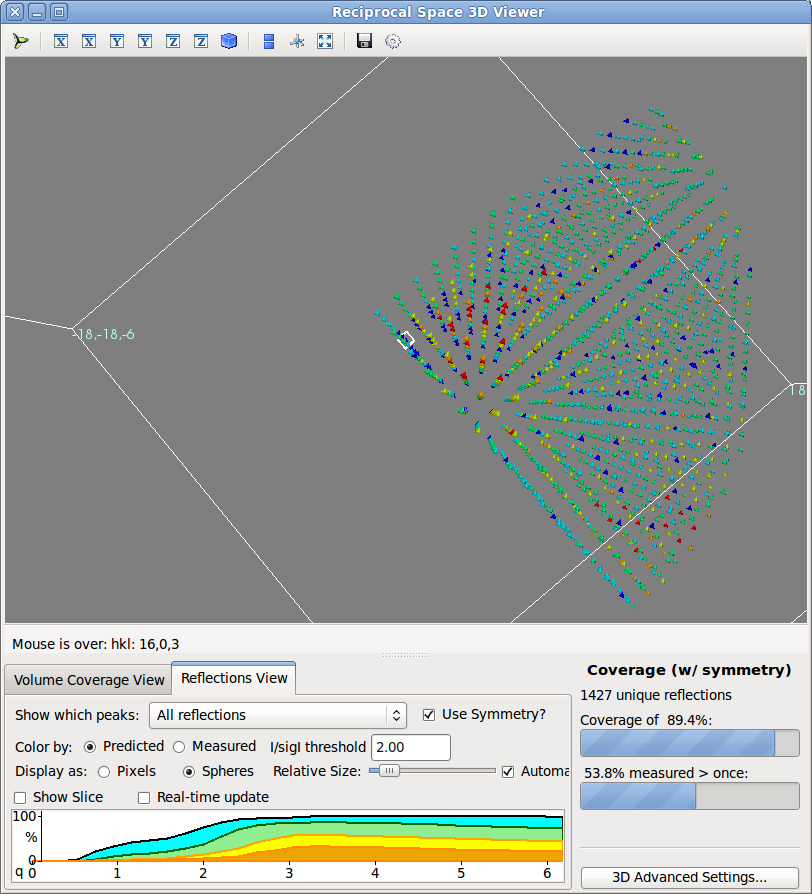
\includegraphics{refl_sym}
\fi
b)
\label{fig:refl_view}
\end{figure}

\begin{figure}
\caption{Part of a GUI showing details of the predicted measurement positions
for a single $hkl$ and some of its equivalents.}
\ifdograph
  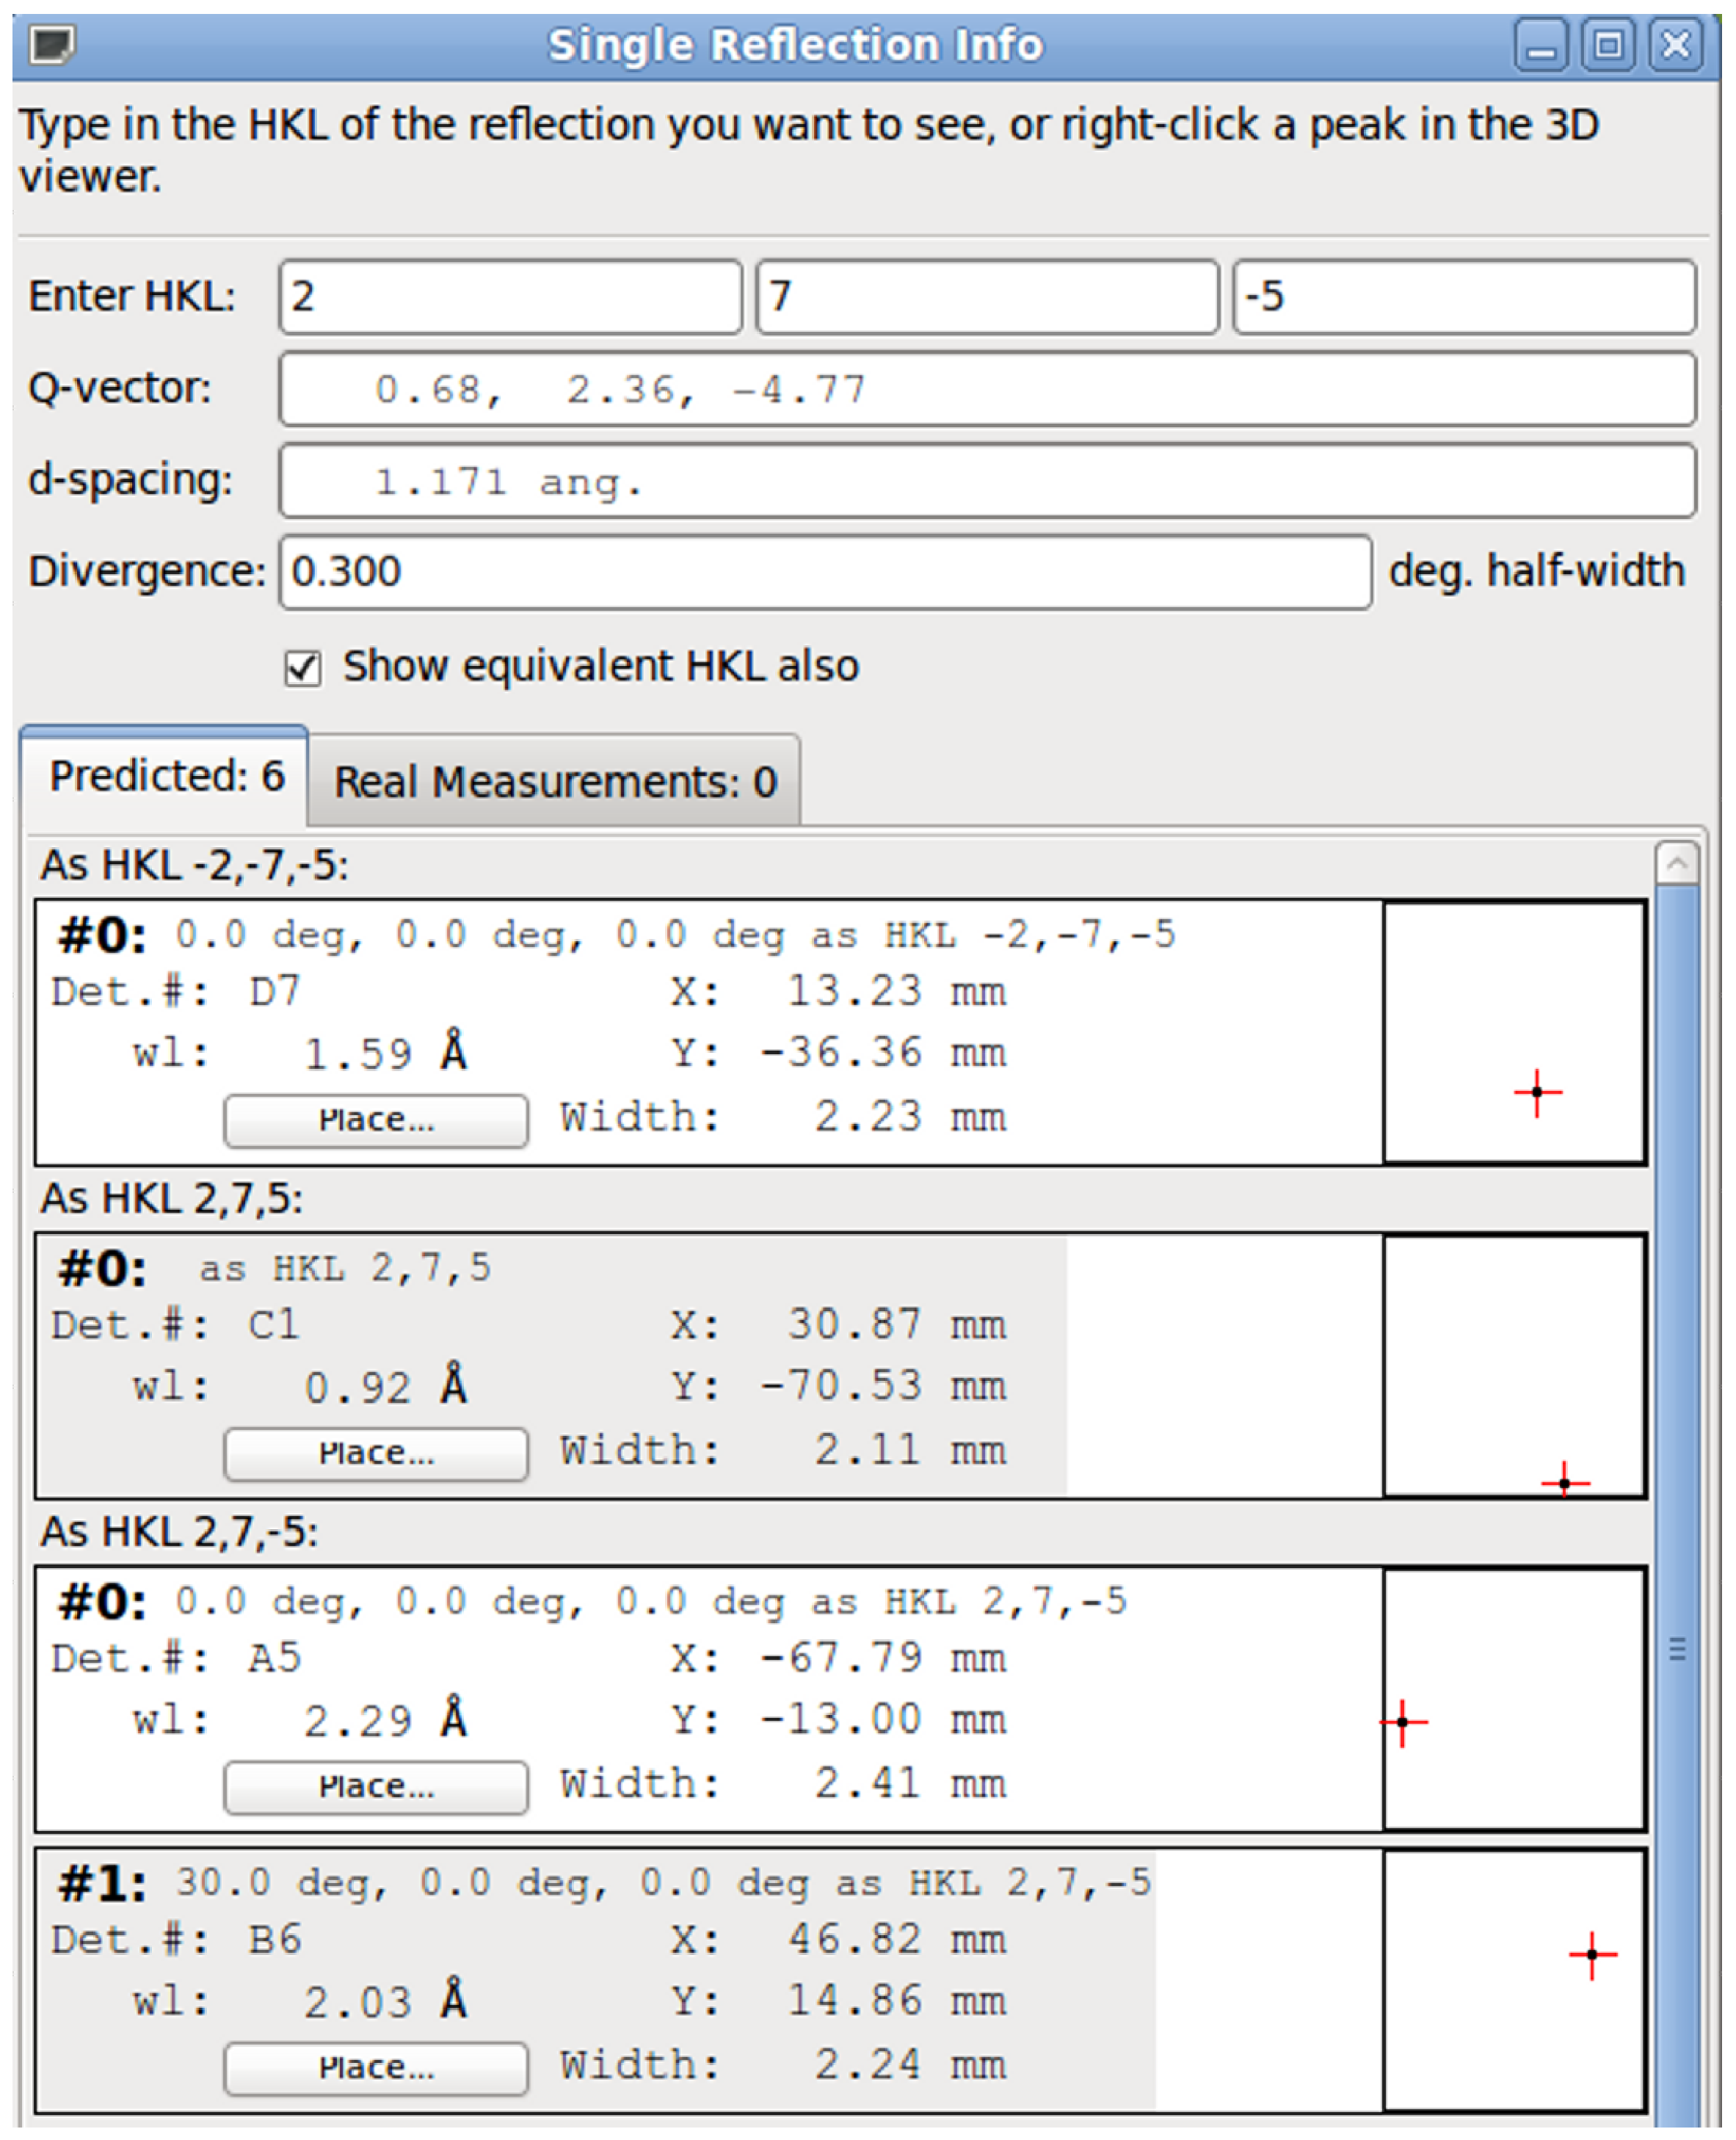
\includegraphics[width=3in]{single_reflection_3}
\fi

\label{fig:single_reflection} 
\end{figure}  
 
  
\begin{figure} 
\caption{a) Screenshot of the Natrolite experiment plan generated using the
Automatic coverage Optimizer. b) Screenshot of the resulting coverage
statistics.}
\ifdograph
  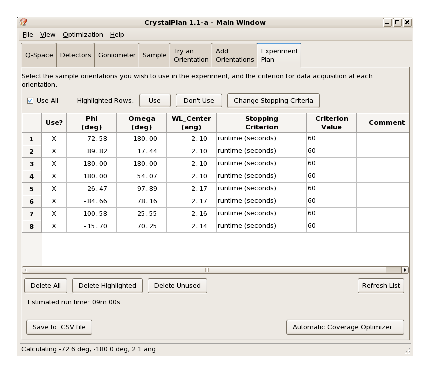
\includegraphics[width=3.5in]{Plan8List}
\fi
a)
\ifdograph
  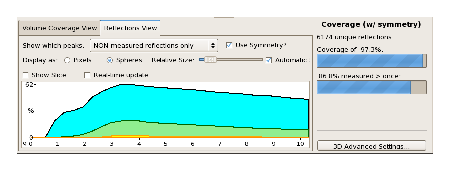
\includegraphics[width=3.5in]{NatCoverage}
\fi
b)
\label{fig:natrolite_gui}
\end{figure}


\end{document}                    % DO NOT DELETE THIS LINE
%%%%%%%%%%%%%%%%%%%%%%%%%%%%%%%%%%%%%%%%%%%%%%%%%%%%%%%%%%%%%%%%%%%%%%%%%%%%%%
